% Options for packages loaded elsewhere
\PassOptionsToPackage{unicode}{hyperref}
\PassOptionsToPackage{hyphens}{url}
%
\documentclass[
]{article}
\usepackage{amsmath,amssymb}
\usepackage{iftex}
\ifPDFTeX
  \usepackage[T1]{fontenc}
  \usepackage[utf8]{inputenc}
  \usepackage{textcomp} % provide euro and other symbols
\else % if luatex or xetex
  \usepackage{unicode-math} % this also loads fontspec
  \defaultfontfeatures{Scale=MatchLowercase}
  \defaultfontfeatures[\rmfamily]{Ligatures=TeX,Scale=1}
\fi
\usepackage{lmodern}
\ifPDFTeX\else
  % xetex/luatex font selection
\fi
% Use upquote if available, for straight quotes in verbatim environments
\IfFileExists{upquote.sty}{\usepackage{upquote}}{}
\IfFileExists{microtype.sty}{% use microtype if available
  \usepackage[]{microtype}
  \UseMicrotypeSet[protrusion]{basicmath} % disable protrusion for tt fonts
}{}
\makeatletter
\@ifundefined{KOMAClassName}{% if non-KOMA class
  \IfFileExists{parskip.sty}{%
    \usepackage{parskip}
  }{% else
    \setlength{\parindent}{0pt}
    \setlength{\parskip}{6pt plus 2pt minus 1pt}}
}{% if KOMA class
  \KOMAoptions{parskip=half}}
\makeatother
\usepackage{xcolor}
\usepackage[margin=1in]{geometry}
\usepackage{graphicx}
\makeatletter
\def\maxwidth{\ifdim\Gin@nat@width>\linewidth\linewidth\else\Gin@nat@width\fi}
\def\maxheight{\ifdim\Gin@nat@height>\textheight\textheight\else\Gin@nat@height\fi}
\makeatother
% Scale images if necessary, so that they will not overflow the page
% margins by default, and it is still possible to overwrite the defaults
% using explicit options in \includegraphics[width, height, ...]{}
\setkeys{Gin}{width=\maxwidth,height=\maxheight,keepaspectratio}
% Set default figure placement to htbp
\makeatletter
\def\fps@figure{htbp}
\makeatother
\setlength{\emergencystretch}{3em} % prevent overfull lines
\providecommand{\tightlist}{%
  \setlength{\itemsep}{0pt}\setlength{\parskip}{0pt}}
\setcounter{secnumdepth}{-\maxdimen} % remove section numbering
\ifLuaTeX
  \usepackage{selnolig}  % disable illegal ligatures
\fi
\usepackage[]{biblatex}
\addbibresource{ReferencesProject1.bib}
\IfFileExists{bookmark.sty}{\usepackage{bookmark}}{\usepackage{hyperref}}
\IfFileExists{xurl.sty}{\usepackage{xurl}}{} % add URL line breaks if available
\urlstyle{same}
\hypersetup{
  pdftitle={Assignment 1},
  hidelinks,
  pdfcreator={LaTeX via pandoc}}

\title{Assignment 1}
\author{}
\date{\vspace{-2.5em}}

\begin{document}
\maketitle

\section{Introduction}\label{introduction}

Portugal has been long celebrated for its wine production, from port
wine to \emph{vino verde} from the Minho province. To address growing
demand, the wine industry is interested in optimising its wine
production. As wine is a food product, most of its prized features are
taste and aroma, which are subjective measurements. Previous studies
have tried to categorise wine by quality through combining human taste
testers, physicochemical analysis and statistical methods in attempts to
introduce objectivity\footnote{\textcite{RN1}}. In this project, we are
most concerned with which \textbf{particular variables} are essential
for considering wine quality. By knowing which variables should be
prioritised, this can motivate further study on optimising the wine
according to essential attributes and enforce more efficient production.

Therefore, this report aims to address the following questions:

\begin{enumerate}
\def\labelenumi{\arabic{enumi}.}
\tightlist
\item
  Which variables play a significant role in ascertaining the quality of
  red and white wine?
\item
  Are there any trends between wine attributes and its perceived
  quality?
\item
  Are there any differences between mean acidity values of wine?
\item
  Are there any differences between mean sulfate/sulfur dioxide values
  of wine?
\end{enumerate}

The dataset employed in this study comprises data sourced from
laboratory tests, providing an intricate look into the chemical
composition of wines from Portugal's Minho region. It encompasses a
comprehensive range of variables, including fixed acidity, volatile
acidity, citric acid, residual sugar, chlorides, free sulfur dioxide,
total sulfur dioxide, density, pH levels, sulphates, alcohol content,
and a subjective quality rating on a scale of 0 to 10, where 10
represents the highest quality. Additionally, a color indicator, as a
dummy variable, distinguishes between red and white wines. - Data
checked for outliers - Total size is 6497 - To account for outliers but
also not to lose too much data, 5\% was chosen (325) entries as max
threshold to lose - Applied a IQR check. Normally, data less than Q1 -
IQR\emph{1.5 or more than Q3 + 1.5 }IQR is common procedure as it does
not assume normality - However, this lead to a large amount fo data
being lost, so stricter threshold of 2.5 was chosen instead.

\subsection{EDA - How does citric acid play a role in quality of
wines?}\label{eda---how-does-citric-acid-play-a-role-in-quality-of-wines}

\begin{itemize}
\tightlist
\item
  Citric acid plays a vital role in wine production
\item
  It helps add freshness to the wine, allowing more lively and enjoyable
  tasting experience, but too much makes it harsh, difficult to
  drink\footnote{\textcite{RN3}}
\item
  Therefore, we are interested in any trends between citric acid
  concentration and perceived wine quality
\item
  Question: Specific to wines of the minho region, what ranges of
  concentrations is related to wine quality?
  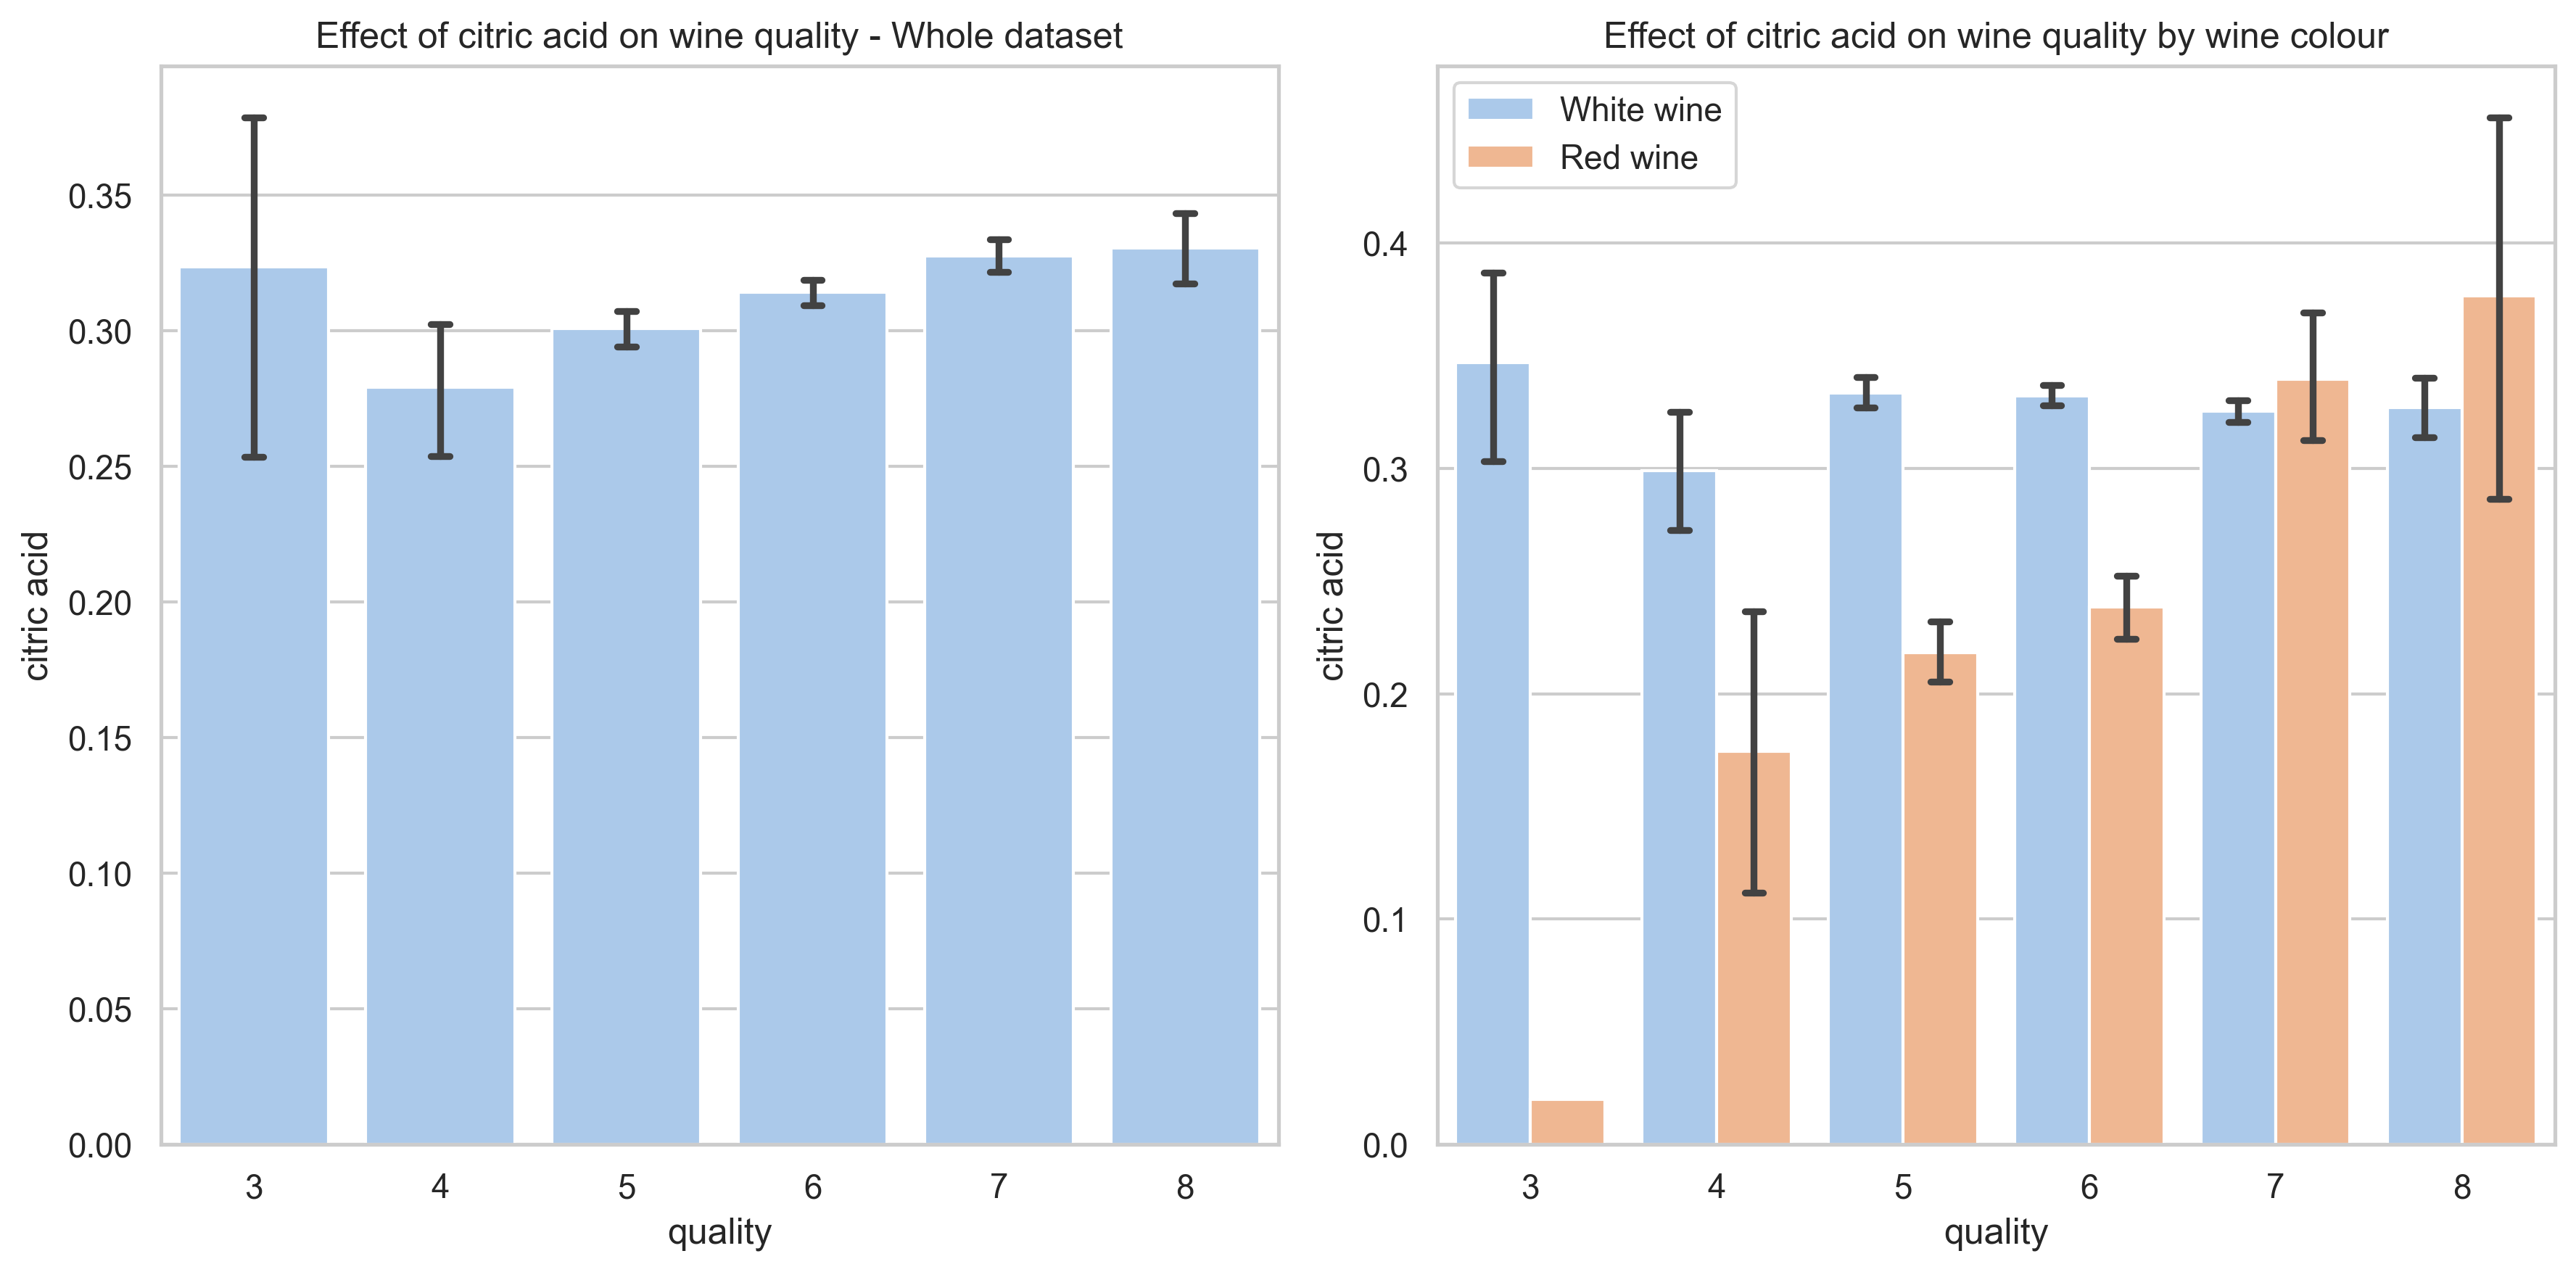
\includegraphics{whole_data_by_colour_citric_acid_vs_quality.png}
\item
  Across dataset:

  \begin{itemize}
  \tightlist
  \item
    High citric acid for low quality (but not certain due to low numbers
    in category 3 and large error bar)
  \item
    Steady increase from quality 4 to 8, but plateaus around 0.33
    g/dm\(^3\)
  \item
    Wines that are ``high quality'' tend to have citric acid
    concentrations between 0.30 g/dm\(^3\) and 0.35 g/dm\(^3\)
  \end{itemize}
\item
  Between wine groups:

  \begin{itemize}
  \tightlist
  \item
    In general, citric acid concentration over higher quality white wine
    seems to be fairly consistent, around 0.30 g/dm\(^3\) and 0.35
    g/dm\(^3\)
  \item
    Red wine much more drastic. Even after accounting for large error
    bars from smaller datapoints for red wine, there is a clear increase
    between higher quality wines have more citric acid
  \end{itemize}
\item
  Conclusion: It seems that higher quality red wines have more citric
  acid in them, but it is unclear whether red wine quality of 9 or
  higher will have more citric acid due to the large error bars. What is
  apparent is higher quality wines in general tend to have citric acid
  concentrations between 0.30 to 0.35 g/dm\(^3\). This disparity could
  be explained by how white wines tend to have more residual sugar than
  red wines, where adding some freshness is more necessary to balance
  out the additional sweetness.\footnote{\textcite{RN1}}
\end{itemize}

\subsection{PCA - Chemical differences between red and white
wines}\label{pca---chemical-differences-between-red-and-white-wines}


\includegraphics{Scree_plot.png} Looking at the scree plot, the elbow
appears around n = 3 components, so we will use this when proceeding
with our PCA model. When considering the key chemical differences
between red and white wines, we need to identify which features produce
large loadings for our model. These features will help maximumise the
langrange multiplier, producing the largest variance which is essential
in differentiating the chemical differences between red and white wines.
!(biplots\_combined){[}biplots\_combined.png{]} From the principal
component plots, the key insights from the loadings we can observe are:
- PC1: Chlorides - Moderate and positive, Volatile acidity - Large and
positive, Colour - large and positive, Sulphates - moderate and
positive, pH - moderate and positive, total sulfur dioxide - moderate
and negative - PC2: Density - Large and positive, Alcohol - large and
negative, Free sulfur dioxide - moderate and positive, Residual sugar -
large and positive - PC3: Fixed acidity - large and positive, Citric
acid - large and positive, colour - close to zero, pH - large and
negative

Insights:

\begin{enumerate}
\def\labelenumi{\arabic{enumi}.}
\tightlist
\item
  Colour is coded as 1 with red wine. Since colour is large and
  positive, red wines will score more highly for PC1. Therefore, we can
  determine that red wines are associated with higher volatile acidity,
  sulphates, pH and total sulfur dioxide. We can confirm this by looking
  through the dataset:
\end{enumerate}

\begin{itemize}
\tightlist
\item
  Chlorides: Most of red wines (min: 0.012, Q1: 0.069, median: 0.078,
  Q3: 0.087, max: 0.132 ) g(sodium chloride)/dm\(^3\) have higher
  chloride values than white wine (min: 0.009, Q1: 0.036, median: 0.043,
  Q3: 0.050, max: 0.132 ) g(sodium chloride)/dm\(^3\)
\item
  Volatile acidity: Most of red wines (min: 0.12, Q1: 0.395, median:
  0.52, Q3: 0.62, max: 0.825 ) g(acetic acid)/dm\(^3\) have higher
  volatile acidity values than white wine (min: 0.08, Q1: 0.210, median:
  0.26, Q3: 0.32, max: 0.815 ) g(acetic acid)/dm\(^3\)
\item
  Sulphates: Most of red wines (min: 0.37, Q1: 0.55, median: 0.61, Q3:
  0.71, max: 1.02 ) g(potassium sulphate)/dm\(^3\) have higher sulphate
  values than white wine (min: 0.22, Q1: 0.41, median: 0.47, Q3: 0.55,
  max: 1.01 ) g(potassium sulphate)/dm\(^3\)
\item
  pH: Most of the red wines (min: 2.88, Q1: 3.24, median: 3.33, Q3:
  3.41, max: 3.78 ) have higher pH values than white wine (but
  marginally) (min: 2.72, Q1: 3.09, median: 3.18, Q3: 3.28, max: 3.82 )
\item
  Total sulfur dioxide: Most the red wines (min: 6.0, Q1: 23.0, median:
  38.0, Q3: 63.0, max: 289.0 ) have much lower total sulfur dioxide
  values than white wines (min: 9.0, Q1: 108.0, median: 134.0, Q3:
  167.0, max: 344.0 )
\end{itemize}

\begin{enumerate}
\def\labelenumi{\arabic{enumi}.}
\setcounter{enumi}{1}
\item
  Wine is produced by fermenting sugar and residual sugar decreases with
  more fermentation. Furthermore, adding sugar or salt to a liquid makes
  it denser. As the alcohol value is large and negative, this means
  wines with less alcohol will have higher PC2 scores. Therefore, this
  component is associated with the age of the wine. While this component
  is not used for chemical differences between red and white wines, this
  will be useful later when considering the quality of the wines.
\item
  Colour does not affect the PC3 score as it is close to zero.
  Furthermore, the group does not appear to be associated with a
  particular red/white wine group. Wines with higher citric acid have
  higher PC3 scores (tends to be white wine, (min: 0.0, Q1: 0.27,
  median: 0.315, Q3: 0.38, max: 0.74) g/dm\(^3\) compared to red wine
  (min: 0.0, Q1: 0.09, median: 0.24, Q3: 0.38, max: 0.73) g/dm\(^3\) ).
  In contrast, wines with high fixed acidity (tends to be red wine) and
  low pH also score highly (Mostly white wine). However, this group
  could be associated with grape harvest time, as studies have suggested
  a relationship between early/late harvest of grapes and grape acidity
  from citric acid and tartaric acid. More research would be needed to
  confirm this.\footnote{\textcite{RN4}}
\end{enumerate}

\textbf{Conclusion}: The main chemical differences between red and
whites are that red wines will have higher chloride, volatile acidity,
sulphates, pH than white wines, but lower total sulfur dioxide and
citric acid concentrations.

\subsection{PCA - Attributes present in wines of high
quality}\label{pca---attributes-present-in-wines-of-high-quality}

To help with visu

\begin{enumerate}
\def\labelenumi{\arabic{enumi}.}
\tightlist
\item
  Plots of principle components
\item
  Comment on the main chemical differences between red and white wines
\item
  Including quality variable what features are likely to be present in
  wines of good quality? Is it different for red and white?
\end{enumerate}

Your research question show address the following: ``What features are
most influential on a particular type of wine of high quality?'' You
should also consider the main chemical differences between red and white
wines (Use the PCA components for this)

\section{One page - Hotelling T square
test}\label{one-page---hotelling-t-square-test}

\begin{enumerate}
\def\labelenumi{\arabic{enumi}.}
\tightlist
\item
  Perform a Hotelling's \(T^2\) -test to test the hypothesis that the
  red and while wines have the same acidity means (the variables fixed
  acidity, volatile acidity and pH)
\item
  Select some variables and compute \(\mu_W\) of selected variables for
  white wine
\item
  Perform 1-sample \(T^2\) test to check whether corresponding means for
  red wine dataset are equal to \(\mu_W\)
\end{enumerate}

\subsection{Approaching the Hotelling T square
test}\label{approaching-the-hotelling-t-square-test}

\begin{enumerate}
\def\labelenumi{\arabic{enumi}.}
\tightlist
\item
  Give a sentence or two for motivation of test
\item
  Give a little math background
\item
  State the hypothesis clearly
\item
  Perform test
\item
  State the result with a confidence interval if applicable
\end{enumerate}

Your report should have: 1. A question stated clearly 2. Explaining the
statistical test used to address question 3. Give solution 4.
Potentially visualisation

Other notes: 1. You must give references 2. Try to keep it to 4 pages

\subsection{Things to keep in mind}\label{things-to-keep-in-mind}

\begin{itemize}
\tightlist
\item
  Citric acid and residual sugar levels are more important in white
  wine, where the equilibrium between the freshness and sweet taste is
  more appreciated
\item
  volatile acidity has a negative impact on wine taste, as it introduces
  bitterness (cite this)
\item
  Sulphastes might link to wine aroma
\item
  Additional research into impact of what affects wine tastes could
  prove useful.
\end{itemize}

Sulphates formed from fermentation. More fermentation =\textgreater{}
more age =\textgreater{} more quality?

\printbibliography

\end{document}
